% testProcedure.tex
\subsection{Source Code Repository}
PR37 MS7 arm uses a different architecture than MS5/6 arm. The branch of each repository is listed below:
\begin{itemize}
	\item keos: release/1.8
	\item bitwin: development (commit ID: 971e7b7, small changes on feature/SWPreleaseKit3\_CTRL\_Update)
	\item rtcontrol\_nextgen: feature/UpdateControlCOnfigFunction
	\item sdk\_assitive: feature/SWPrelease\_CTRL\_Update
\end{itemize}

\subsection{Data acquisition}
\begin{enumerate}
	\item run executable rtcontrol on QNX
	\item run sdk\_assitive to get NOVA interface on PC (as in Figure \ref{fig:nova})
	\item select AURIS in NOVA
	\item select AURIS Control in NOVA
	\item set IP of QNX, Run Mode in "run", and then click Connect
	\item release robot break
	\item input a pre-defined robot configuration in Custom Configuration in NOVA and send it to robot
	\item click Live Data to view data in real time
	\item make a screenshot of Live Data to collect data
	\item input a new pre-defined robot configuration and repeat the steps to get data for all pre-defined robot configurations
\end{enumerate}

\begin{figure}
	\begin{center}
		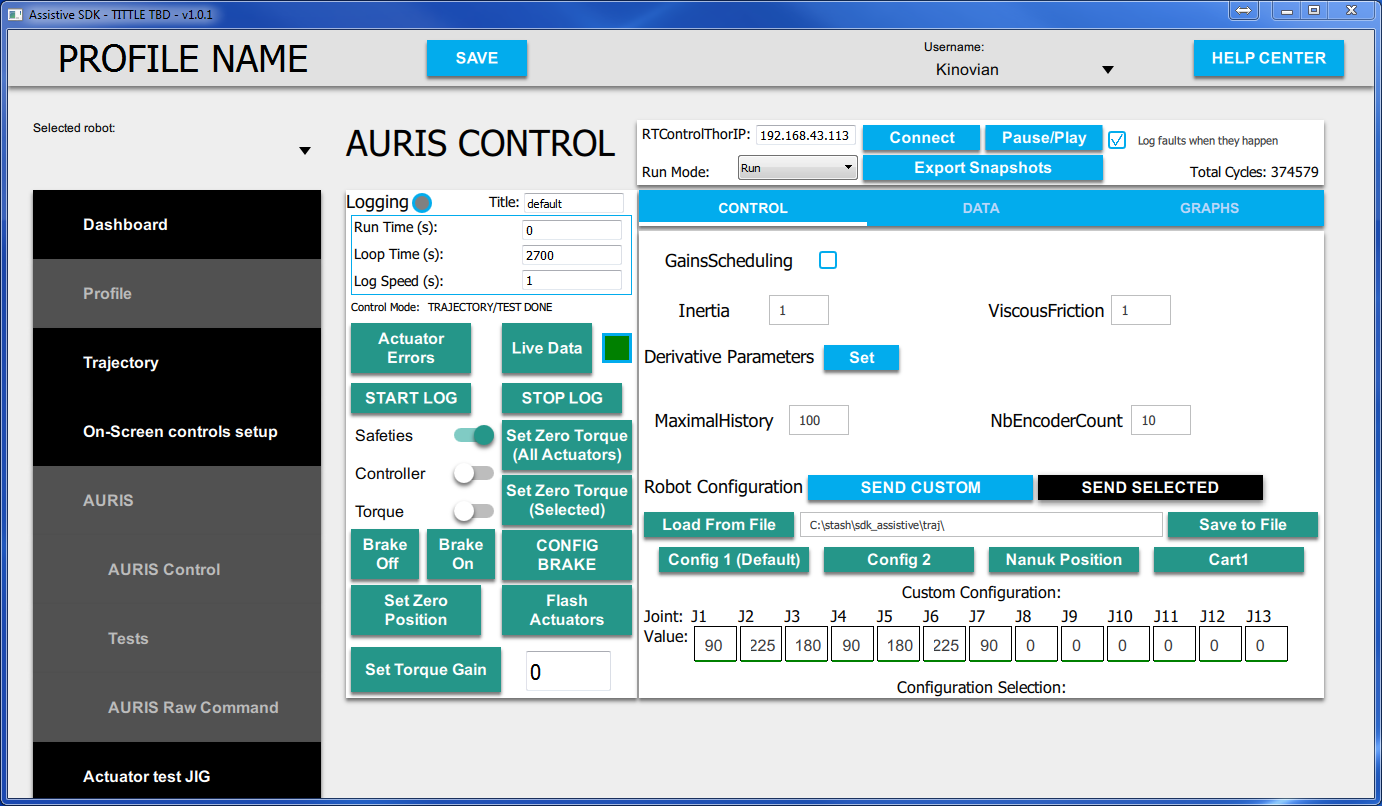
\includegraphics[width=0.9\textwidth]{./images/NOVA}%
		\caption{NOVA interface}
		\label{fig:nova}%
	\end{center}
\end{figure}
